\begin{figure*}%
	\centering%
	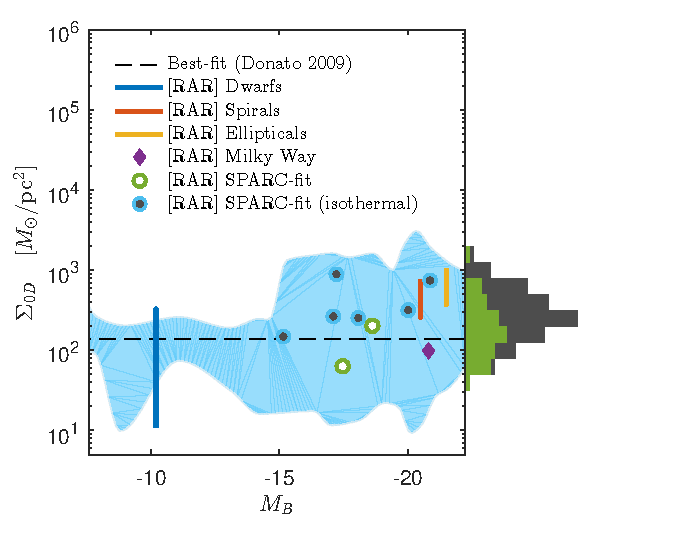
\includegraphics[width=\hsize]{\ROOTPATH/fig.pdf}
	\caption{$\chi^2$ profiles for NGC6015. This galaxy is characterized through an extended halo tail with oscillations. This \textit{abundance} of information in the outer halo region clearly favors isothermal halos, corresponding to relatively high cutoff values. Those solutions provide extended halo tails with a wide halo maximum, suitable but insufficient for fitting well the rotation curve. Solutions with lower $W_0$ values are ruled out according to this analysis. The latter corresponds here to profiles with contracted halos without developing isothermal tails due to surface effects.}%
	\label{fig:NGC6015:deep-chi2}%
\end{figure*}